% -----------------------------------------------
% Template for ISMIR LBD Papers
% 2024 version, based on previous ISMIR templates

% Requirements :
% * 2+1 page length maximum
% * 10MB maximum file size
% * Copyright note must appear in the bottom left corner of first page
% * Clearer statement about citing own work in anonymized submission
% (see conference website for additional details)
% -----------------------------------------------

\documentclass{article}
\usepackage[T1]{fontenc} % add special characters (e.g., umlaute)
\usepackage[utf8]{inputenc} % set utf-8 as default input encoding
\usepackage{ismir,amsmath,cite,url}
\usepackage{graphicx}

\usepackage{color}
\usepackage[ruled,noend,linesnumbered]{algorithm2e}


% Add watermark for LBD
\usepackage[firstpage]{draftwatermark}
\definecolor{lightgray}{rgb}{0.9,0.9,0.9}
\definecolor{darkgray}{rgb}{0.4,0.4,0.4}
\SetWatermarkFontSize{12pt}
\SetWatermarkScale{1.1}
\SetWatermarkAngle{90}
\SetWatermarkHorCenter{202mm}
\SetWatermarkVerCenter{170mm}
\SetWatermarkColor{darkgray}
\SetWatermarkText{Late-Breaking / Demo Session Extended Abstract, ISMIR 2024 Conference}


\newcommand{\code}{\texttt}

\def\lbd{}	% Flag to use correct LBD settings in the paper, please do not modify this line

\usepackage{lineno}
\linenumbers


% \onecolumn
% Title. Please use IEEE-compliant title case when specifying the title here,
% as it has implications for the copyright notice
% ------
\title{Zero-shot Crate Digging $\rightarrow$ DJ Tool retrieval using \{Speech, Music\} Activity and CLAP embeddings}

% Note: Please do NOT use \thanks or a \footnote in any of the author markup

% Single address
% To use with only one author or several with the same address
% ---------------
\oneauthor
 {Iroro Orife}
 {{\tt iroro@alumni.cmu.edu}}

% Two addresses
% --------------
%\twoauthors
%  {First author} {School \\ Department}
%  {Second author} {Company \\ Address}

% Three addresses
% --------------
%\threeauthors
%  {First Author} {Affiliation1 \\ {\tt author1@ismir.edu}}
%  {Second Author} {\bf Retain these fake authors in\\\bf submission to preserve the formatting}
%  {Third Author} {Affiliation3 \\ {\tt author3@ismir.edu}}

% Four or more addresses
% OR alternative format for large number of co-authors
% ------------
%\multauthor
%{First author$^1$ \hspace{1cm} Second author$^1$ \hspace{1cm} Third author$^2$} { \bfseries{Fourth author$^3$ \hspace{1cm} Fifth author$^2$ \hspace{1cm} Sixth author$^1$}\\
%  $^1$ Department of Computer Science, University , Country\\
%$^2$ International Laboratories, City, Country\\
%$^3$  Company, Address\\
%{\tt\small CorrespondenceAuthor@ismir.edu, PossibleOtherAuthor@ismir.edu}
%}

% For the author list in the Creative Common license and PDF metadata, please enter author names. 
% Please abbreviate the first names of authors and add 'and' between the second to last and last authors.
\def\authorname{I. Orife}

% Optional: To use hyperref, uncomment the following.
%\usepackage[bookmarks=false,pdfauthor={\authorname},pdfsubject={\papersubject},hidelinks]{hyperref}
% Mind the bookmarks=false option; bookmarks are incompatible with ismir.sty.

\sloppy % please retain sloppy command for improved formatting

\begin{document}

%
\maketitle
%
\begin{abstract}
In genres like Hip-Hop, RnB, Reggae, Dancehall and just about every Electronic/Dance/Club style, DJ tools are a special set of audio files curated to heighten the DJ's musical performance and creative mixing choices. In this work we demonstrate an approach to discovering DJ Tools in personal music collections. Given a large set of audio files in a personal or DJ music library, we utilize zero-shot audio classification on audio segments created from music structure boundary analysis and speech and music activity. The system offer a novel way for DJs to rediscover tools in their personal music collections.
 \end{abstract}
%
\section{Introduction}\label{sec:introduction}
Whether mixing live or in the studio, DJ tools facilitate creative mixing options for remixes, re-edits, re-drums, mashups, long-playing mixtapes, etc. Tools vary by genre and era, but are generally short, simplified musical phrases retrieved from existing music with the intention to reuse in a DJ performance. These musical phrases range from sound effects to acapella loops to purely instrumental passages, solo percussion or drum break to an entire verse or bridge of song. For example a DJ might trigger an acapella loop or long sound effect while mixing a transition from SongA $\rightarrow$ SongB. DJ Tools are commonly sold in online shops along with royalty-free sound libraries, samplepacks of loops and beats. Most tools include key signature, beat and tempo metadata where necessary to ensure sync to the DJ project master tempo.

\subsection{Crate digging \& a short history of DJ tool}\label{sec:history}

Before the advent of online shops trading sonic tool, DJs and producers were known to spend time in record shops crate-digging, or hunting for rare, vintage, or otherwise obscure vinyl with interesting breaks, melodic hooks, drops, intros/outros, or B-side acapellas. Practise time was devoted to studying the structure of music, identifying suitable mix points, curating tools and experimenting with different creative interpolations between two mixable songs. Then while playing live, tools are triggered or looped from Sampler modules or ``Remix Decks'' connected to the DJ mixing board.

\subsection{Musical structure, speech activity and zero-shot classification}\label{sec:djtool_classes}
DJ tools naturally occur at moments in a song where there is a transition to a simpler, less-dense mix. Ergo, we leverage the music structural analysis framework (MSAF) boundary detection algorithms to supply approximate time-offsets of structural progressions \cite{nieto2016systematic}. Next, we employ a speech and music activity detector (SMAD)\cite{Hung2022} to further refine which passages to gather for classification.

For DJ-tool classification we engage the zero-shot capabilities of a Contrastive Language-Audio Pretraining (CLAP) model \cite{elizalde2022claplearningaudioconcepts}. Given an audio segment $X^{a}$ and a list of text descriptions of different DJ tool classes \{$X^{t}_{1},...,X^{t}_{M}$\}, we use CLAP's pretrained \{audio, text\} encoders and their projection layers to compute CLAP embeddings $E^a$ and $E^t_i$. The classification logits $D_i$ can be computed as magntidue of the cosine similarity between the audio segment embedding and \textit{each} text embedding.

\begin{equation}
\begin{matrix}
    X^{a} \rightarrow AudioEncoder \rightarrow E^{a} \\ 
    \{X^{t}_{1},...,X^{t}_{M}\} \rightarrow TextEncoder \rightarrow \{E^{t}_{1},...,E^{t}_{M}\} \\ 
\end{matrix}
\end{equation}

\begin{equation}
    D_i = Similarity(E^a, E^{t}_{i}) \\ 
\end{equation}


\begin{figure}
 \centerline{
 	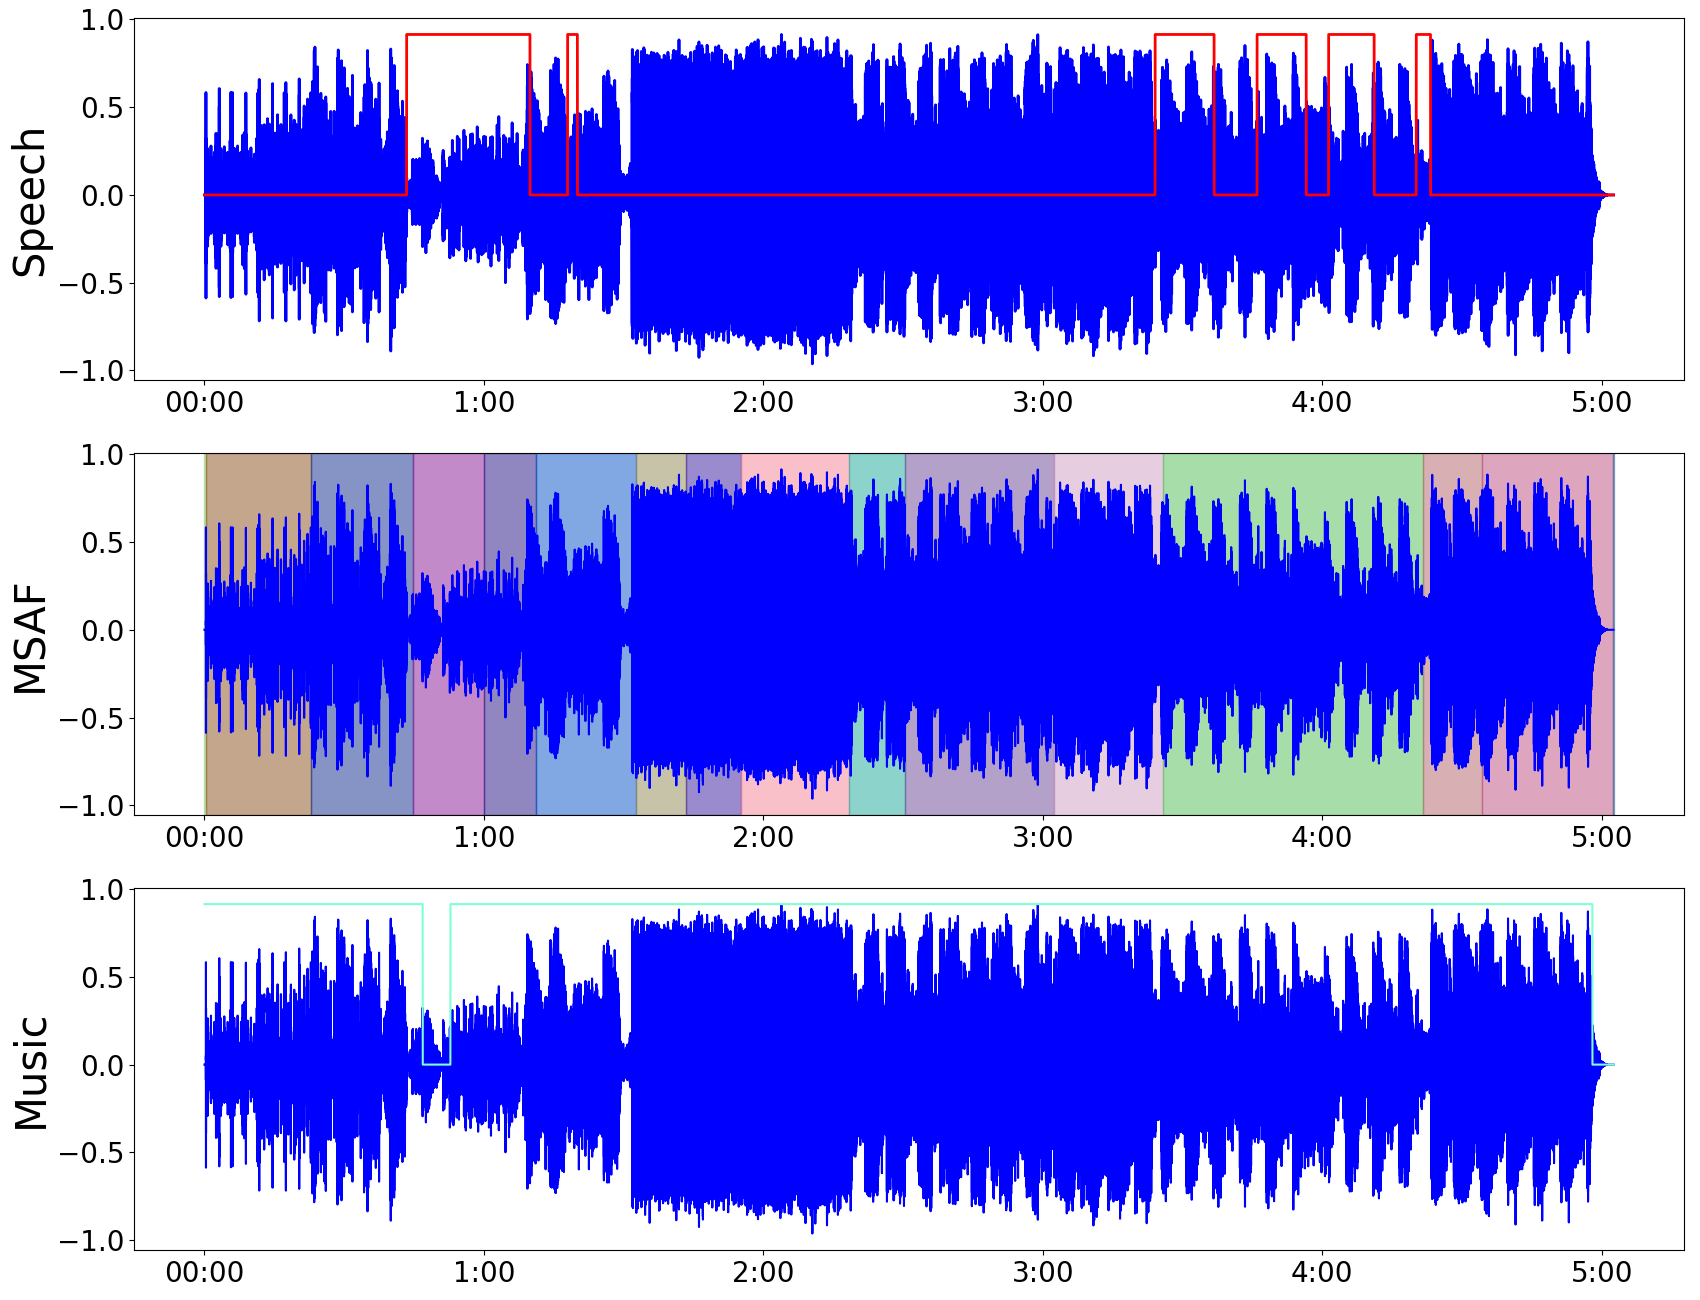
\includegraphics[alt={SMAD \& MSAF Analysis signals},width=0.9\columnwidth]{smad_msaf.png}}
 \caption{A 5 minute Ragga Jungle song overlaid with detected speech and music activity, as well as music-structural boundaries}
 \label{fig:msafsmadplot}
\end{figure}


\section{The System}\label{sec:system}

The system is based on fully open-source Python tools. Firstly, MSAF\footnote{https://github.com/urinieto/msaf} and SMAD\footnote{https://github.com/biboamy/TVSM-dataset/tree/master} are run independently to generate raw activities and structural boundaries saved as CSV files. Next, these are post-processed to yield two lists of time ranges or ``time windows'' and a list of boundary-times. In principle, we can just use the boundary times to segment the song, however if we use the speech onset times from SMAD, we can get a more accurate onset time for the region. Figure \ref{fig:msafsmadplot} shows the relationship between the boundaries and the speech activity. 

Next, for zero-shot classification we use the LAION version of CLAP hosted on Huggingface\footnote{https://huggingface.co/laion/clap-htsat-unfused}

The source code\footnote{https://github.com/ruohoruotsi/djtool-crate-digging} is fully open source, relying only on open-source libraries and models. Interested users can use the main Python file to retreive DJ Tools in their personal music libraries.


\subsection{Algorithm}\label{subsec:algo}
Below we outline how we go about procesing all files in a music library. Note the term ``window''  below refers to a tuple with the following temporal attributes $\rightarrow$ \code{start\_time, end\_time, label}

\begin{algorithm}
    \caption{Zero-shot Crate Digging}\label{combo_algo}
    	Create text prompts for $M$ classes \{$X^{t}_{1},...,X^{t}_{M}$\} \\
    	 $\{E^{t}_{1},...,E^{t}_{M}\} \gets TextEncoder(\{X^{t}_{1},...,X^{t}_{M}\})$ \\
		\BlankLine

        \For{song $s_i$ in the library $S_N$}{
            $W^{s}, W^{m} \gets SMAD(s_i)$ \\ 
            $B \gets MSAF(s_i)$  \\
            Adjust boundaries $B_i$ to nearest $W^{s}$ \\
			Use $B$ to cut $s_i$ to audio files \{$X^a_1$,..., $X^a_N$\} \\
		    \BlankLine
            \For{$j := $1 to $N$}{
                $E^{a}_j \gets AudioEncoder(X^a_j)$ \\
                $D_{j_i} \gets Similarity(E^a_j, E^{t}_{i})$ \\
                Bucket each $D_{j_i}$ into one of $M$ classes \\
                Save audio file \& predicted class metadata \\
                \BlankLine
            }
        }
\end{algorithm}

\subsection{Results or Experience using the system}

\begin{table}
 \begin{center}
 \begin{tabular}{|l|l|}
  \hline
  DJ Tool class & Example description text prompt \\
  \hline
	Acapella loops & ``expressively sung vocal tracks''  \\
	Sound effects &  ``siren, riser sound effects''\\
	Drums breaks  & ``drum beat, drum solo, breakbeat''  \\
	Melodic hooks & ``solo guitar, piano melody''  \\
	DJ Drops & ``Massive EDM drop''  \\
	Battle tracks & ``vinyl scratch loop, turnatablist''   \\
	... & ... \\
  \hline
 \end{tabular}
\end{center}
 \caption{In practise, for each class $C_i$, there are host of valid text-prompts. There is also a bit or art to capture the textual essence of each class}
 \label{tab:example}
\end{table}


\section{Related Work}
There is not much existing work within the community relevant to DJs. The few studies that we could find focused on Pop or EDM genres, which may have less of a crate-digging culture. These works focused on the challenges of ideal sequencing of songs and inter-song transitions with an eye toward the fully automatic DJ \cite{kim2017automatic, huang2017djnet, bittner2017automatic}.

In a recent work from 2023, DJ STRUCTFREAK, the authors tackle the task of carefully choosing suitable ``mix points'' \textit{within} a song to generate smooth, aesthetic transitions \cite{kim2023dj}. Similar to this work, they employ structural analysis and beat and frame-level embeddings \cite{kim2023all}. 


% fully automated system that generates DJ mixes from an arbitrary pool of audio tracks. 





\section{Future Work}

In this work, we demonstrate a simple tool leveraging 3 open-source audio classification libraries, operating on large, personal music libraries for the specific task of retrieval of relevant, DJ-centric audio files for use in live DJ performance. 

Future work includes improving the fidelity of the boundary detection algorithms and exploring a more modern structural segmentation approach like \cite{kim2023all}. If there is enough interest to turn DJ tool retrieval into a proper MIR task, then the first order of future work will be a labeled evaluation dataset. Finally, a front-end UI would be useful for strictly non-programmer Deejays.

% For bibtex users:
\bibliography{ISMIRtemplate}

\end{document}

